%% main.tex — haskell-mnist paper
%% Compile-time dimension safety for a from-scratch MNIST classifier in Haskell.
%%
%% Build: latexmk -pdf main.tex   (or pdflatex + bibtex + pdflatex ×2)
%% Requires the ACM template class (acmart), available on CTAN / Overleaf.
%%
%% [nonacm] removes the ACM rights block / conference footer — appropriate for a
%% course paper. Remove it if a proper ACM submission format is required.
\documentclass[sigconf,nonacm]{acmart}

%% ---- Packages ---------------------------------------------------------------
%% acmart already loads: graphicx, booktabs, hyperref, amsmath (via amsart core).
\usepackage{listings}
\usepackage{tikz}
\usetikzlibrary{arrows.meta, positioning}
\usepackage[capitalise]{cleveref}   % must load after hyperref (acmart loads it)
\crefname{listing}{Listing}{Listings}
\Crefname{listing}{Listing}{Listings}

%% ---- Listings style ----------------------------------------------------------
\lstset{
  basicstyle=\ttfamily\footnotesize,
  breaklines=true,
  frame=single,
  columns=fullflexible,
  keepspaces=true
}

%% ---- Metadata -----------------------------------------------------------------
\title{An Auditable, Type-Indexed MNIST Classifier in Haskell}

\author{Gabriel Bringel Gonçalves}
\affiliation{%
  \institution{Universidade Federal da Paraíba}
  \city{João Pessoa, PB}
  \country{Brazil}}
\email{gbg@academico.ufpb.br}

\begin{document}

%% =============================================================================
%% Abstract
%% =============================================================================
\begin{abstract}
Neural networks are built from tensor operations whose correctness depends on
matching dimensions, and shape mismatches are a documented, recurring class of
fault in deep-learning code. In mainstream frameworks a shape is an ordinary
runtime value, so a mismatched product or an incompatibly composed layer fails
only at execution---late, displaced from its cause, and only on code paths that
are run. Lifting these dimensions into the type system, where the compiler
checks them, is an idea that typed array languages and typed neural-network
libraries in Haskell already realize. We revisit it not as another library but
as a minimal, auditable reconstruction. In this feedforward MNIST classifier the
linear algebra, the forward pass, and a hand-written reverse-mode
backpropagation are all written from scratch---no BLAS, no
automatic-differentiation engine, no external binding---with every vector and
matrix indexed by its size as a type-level natural, so that a length-$n$ vector
has type $\mathtt{Vec}\ n$ and an $r\times c$ matrix has type
$\mathtt{Mat}\ r\ c$. A dimension mismatch is therefore a compile-time error
rather than a runtime crash, and the same discipline extends to the backward
pass, in which each gradient carries the type of the tensor it differentiates,
so the reverse pass is shape-checked exactly as the forward pass is. Because a
well-typed gradient can still be numerically wrong, we verify the hand-derived
gradients \emph{per-element} (component by component) against finite differences
in a property-based test suite of $16$ QuickCheck properties, and, as an
end-to-end confirmation that the typed passes are correct, train the network on
MNIST to $95.49\%$ test accuracy. The contribution is expository: it makes legible and
checkable, in the text of one small program, the shape discipline that
production libraries encapsulate.
\end{abstract}

\maketitle

%% =============================================================================
%% 1. Introduction
%% =============================================================================
\section{Introduction}
\label{sec:introduction}

Neural networks are built from tensor operations---matrix--vector products,
transpositions, elementwise maps---whose correctness depends on the operands'
dimensions lining up exactly. In mainstream frameworks such as NumPy and PyTorch,
those dimensions are ordinary runtime values, and a shape mismatch is caught only
when the offending operation executes~\cite{numpy,pytorch}. The resulting error
is both late and displaced: it surfaces as an exception deep inside a
computation, often far from the line that introduced the wrong shape, and only if
that code path is run at all. This is not a hypothetical failure mode: an
empirical study of deep-learning code finds shape and dimension mismatches among
the most common fault categories~\cite{zhang2018empirical}, and the difficulty of
catching them statically, rather than after the fact, has motivated dedicated
analyses that reconstruct a program's tensor shapes from its framework
code~\cite{lagouvardos2020pythia}.

This runtime character is the root of the problem. Because a tensor's shape is
not part of its type, the compiler cannot see that a $10\times5$ matrix is being
multiplied by a length-$3$ vector; nothing rules out the mismatch until execution
reaches it. For a network, whose every weight, activation, and gradient has a
dimension fixed by the layer sizes, this places an entire class of bug---a
transposed matrix, a layer wired to the wrong-sized input, two layers composed at
a mismatched boundary---outside the reach of static checking. The question this
raises is whether those dimensions can instead be made part of the type, so that
the mismatch never compiles.

In this paper we answer that question by building a complete MNIST classifier in
Haskell whose tensors carry their dimensions in their types. Using type-level
natural numbers (\textsc{DataKinds}), a length-$n$ vector has type
$\mathtt{Vec}\ n$ and an $r\times c$ matrix has type $\mathtt{Mat}\ r\ c$, and
every operation is typed so that only dimension-consistent uses are well-formed:
the matrix--vector product $\mathtt{Mat}\ r\ c \to \mathtt{Vec}\ c \to
\mathtt{Vec}\ r$ ties the vector's length to the matrix's column count.
\Cref{fig:pipeline} shows a single input flowing through the network with its
type changing at each layer. A dimension mismatch is then a type error, reported
at the call site before the program runs (\Cref{lst:dimerror}), rather than a
runtime crash.

%% ---- Figure 1: type-flow pipeline (teaser) ----------------------------------
\begin{figure*}[t]
  \centering
  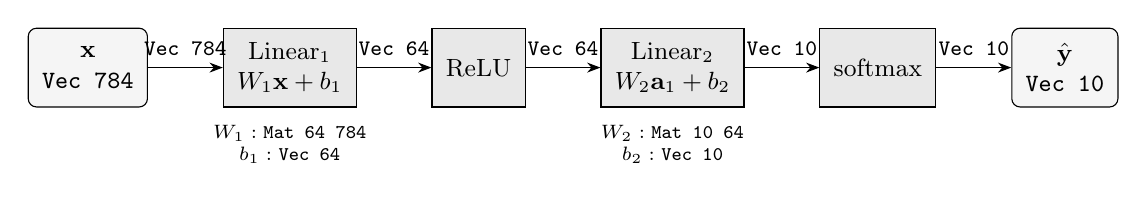
\begin{tikzpicture}[
    >=Stealth,
    font=\small,
    node distance=0.95cm,
    tensor/.style={rounded corners=3pt, draw, fill=gray!8, align=center,
                   inner sep=5pt, minimum height=1cm},
    op/.style={draw, fill=gray!18, align=center, inner sep=5pt,
               minimum height=1cm},
    typelabel/.style={font=\footnotesize\ttfamily, midway, above=1pt},
    paramlabel/.style={font=\scriptsize, align=center, below=3pt}
  ]
    \node[tensor] (x)                      {$\mathbf{x}$\\\texttt{Vec 784}};
    \node[op, right=of x]    (l1)          {Linear$_1$\\$W_1\mathbf{x}+b_1$};
    \node[op, right=of l1]   (relu)        {ReLU};
    \node[op, right=of relu] (l2)          {Linear$_2$\\$W_2\mathbf{a}_1+b_2$};
    \node[op, right=of l2]   (soft)        {softmax};
    \node[tensor, right=of soft] (y)       {$\hat{\mathbf{y}}$\\\texttt{Vec 10}};

    \draw[->] (x)    -- (l1)   node[typelabel]{Vec 784};
    \draw[->] (l1)   -- (relu) node[typelabel]{Vec 64};
    \draw[->] (relu) -- (l2)   node[typelabel]{Vec 64};
    \draw[->] (l2)   -- (soft) node[typelabel]{Vec 10};
    \draw[->] (soft) -- (y)    node[typelabel]{Vec 10};

    \node[paramlabel] at (l1.south) {$W_1:\;$\texttt{Mat 64 784}\\$b_1:\;$\texttt{Vec 64}};
    \node[paramlabel] at (l2.south) {$W_2:\;$\texttt{Mat 10 64}\\$b_2:\;$\texttt{Vec 10}};
  \end{tikzpicture}
  \caption{Type flow through the network. A single input
    $\mathbf{x} : \texttt{Vec 784}$ is threaded through two linear layers and
    their activations to a distribution $\hat{\mathbf{y}} : \texttt{Vec 10}$; the
    monospaced annotation on each edge is the shape of the value passing along
    it, and the parameter types beneath each layer fix its dimensions. Because
    $\mathtt{mulV} : \mathtt{Mat}\ r\ c \to \mathtt{Vec}\ c \to \mathtt{Vec}\ r$
    ties a layer's input length to its weight matrix's column count, only a
    network whose successive dimensions agree---$784, 64, 64, 10, 10$---is
    well-typed.}
  \label{fig:pipeline}
\end{figure*}

The same discipline covers the part of a network most prone to hand-coding
mistakes: the gradients. We write backpropagation by hand, with no
automatic-differentiation library, as a typed reverse pass in which the gradient
of a tensor has the type of that tensor---the gradient of a $\mathtt{Mat}\ r\ c$
is again a $\mathtt{Mat}\ r\ c$. The backward pass is therefore checked by the
type system exactly as the forward pass is, and the shape identities of
backpropagation become visible in the types rather than hidden inside a
differentiation engine (\Cref{sec:backprop}).

We validate the implementation on two fronts. The type-level guarantee is shown
by the compiler rejecting a deliberate mismatch (\Cref{lst:dimerror}), and the
numerical content is verified by a property-based test suite in which the
hand-derived gradients are checked \emph{per-element} against finite
differences. As an end-to-end confirmation that the typed forward and backward
passes are correct, the network trains on MNIST to $95.49\%$ test accuracy with
no automatic differentiation and no BLAS (\Cref{sec:results}).

This project is not another library but a minimal, auditable reconstruction, and
its aim is expository: to make legible, in the text of one small program, the
shape discipline that typed Haskell tensor libraries already encapsulate.
Type-indexed tensors for neural networks are not themselves new---Grenade,
TensorSafe, and Hasktorch all realize them, and Grenade likewise verifies its
backpropagation by finite differences (\Cref{sec:bg:related}). What distinguishes
this work is one of degree, not of concept: it writes the linear algebra, the
forward pass, and the backward pass all by hand on a minimal, fixed-size core,
depending on no linear-algebra library, so that every operation and every
gradient stays legible and finite-difference-verified in the program's own
text.

\paragraph{Contributions.}
In summary, this paper contributes:
\begin{itemize}
  \item a legible, auditable reconstruction of a feedforward MNIST classifier in
    Haskell whose tensor dimensions are type-level naturals, turning every
    dimension mismatch---within an operation or across composed layers---into a
    compile-time error;
  \item a hand-written, typed reverse-mode backpropagation in which each gradient
    carries the type of the tensor it differentiates, so the backward pass is
    shape-checked like the forward pass, with no automatic-differentiation
    library; and
  \item a per-element verification of the hand-derived gradients
    against finite differences, together with an end-to-end functional result
    ($95.49\%$ on MNIST) confirming the typed implementation trains correctly.
\end{itemize}

%% =============================================================================
%% 2. Background
%% =============================================================================
\section{Background}
\label{sec:background}

\subsection{MNIST and feedforward classification}
\label{sec:bg:mnist}

MNIST is a standard benchmark of $28\times28$ grayscale images of handwritten
digits, each labeled with one of ten classes~\cite{lecun-mnist}. A feedforward
classifier maps a flattened image $\mathbf{x}\in\mathbb{R}^{784}$ through a
sequence of affine transformations $\mathbf{z} = W\mathbf{x} + \mathbf{b}$
interleaved with nonlinearities, ending in a probability distribution over the
ten classes. The parameters are fit by minimizing a loss with gradient descent,
and the gradients are obtained by reverse-mode differentiation
(backpropagation): the loss gradient is propagated from the output back through
each layer, reusing intermediate values from the forward pass. The dimensions of
every weight, activation, and gradient are fixed by the network's layer sizes,
and a single transposed matrix or mismatched layer boundary is enough to make the
computation ill-formed---the class of error this work eliminates.

\subsection{Type-level naturals in Haskell}
\label{sec:bg:datakinds}

Our implementation encodes those dimensions in the types, using three GHC
features. \textsc{DataKinds} promotes ordinary natural-number literals to the
type level, so that a size such as $784$ or $10$ can appear as a type
index~\cite{datakinds}. A type parameter of kind $\mathtt{Nat}$ then lets a data
type carry a dimension without storing it: in $\mathtt{Vec}\ (n :: \mathtt{Nat})\
a$, the index $n$ is a phantom that constrains the type but not the runtime
representation. When the size is genuinely needed as a runtime integer---to
allocate a vector, for instance---the $\mathtt{KnownNat}$ class and its
$\mathtt{natVal}$ reflect the type-level $\mathtt{Nat}$ back down to an
$\mathtt{Int}$. Together these turn a dimension into a compile-time quantity that
the type checker can reason about, which is what makes a mismatch a type error
rather than a runtime fault (\Cref{sec:architecture}).

\subsection{Related work}
\label{sec:bg:related}

Work on shape safety for tensor programs spans a spectrum, from checks
performed purely at runtime to checks performed statically, before the program
ever runs. We survey this spectrum in order of increasing static guarantee,
before turning, separately, to how gradients themselves are computed.

\paragraph{Runtime shape verification.}
At the dynamic end of the spectrum, shapes and dtypes are checked purely at
runtime, through type annotations that a checker enforces as the program
executes: jaxtyping and beartype-style checkers validate an array's declared
shape and dtype against its actual value at each call~\cite{kidger2022jaxtyping}.
The check remains dynamic---a mismatch still surfaces only when the annotated
code runs---but it moves the error closer to its cause and reports a legible
message in place of a shape exception raised deep inside an unrelated
operation.

\paragraph{External static analysis.}
Moving a step toward static checking, a separate tool can analyze framework
code before it runs at all: Pythia reconstructs a TensorFlow program's tensor
shapes by static analysis of its operations~\cite{lagouvardos2020pythia}, and
PyTea performs a comparable static analysis of PyTorch training code to flag
shape errors ahead of execution~\cite{jhoo2021pytea}. Both catch many
mismatches before the program runs, but as analyses external to the language,
each is best-effort: unsound or incomplete in general, and separate from the
type checker the programmer already relies on.

\paragraph{Gradual typing in the language.}
A further step brings shape information into the language's own type system,
but only gradually. Variadic generics for Python, standardized as PEP 646, let
a tensor's rank and axis sizes appear as type parameters that an ordinary
static type checker can consult~\cite{pep646}, and shape-aware type checkers
such as Pyrefly propagate and check these annotations across a
codebase~\cite{pyrefly}. The checking is optional and partial: a program is
verified only as far as its annotations reach, and unannotated code passes
through unchecked.

\paragraph{Static types with a dynamic escape hatch.}
Further still, some array languages put sizes in the type system by default
rather than by annotation, while retaining an explicit, controlled way to fall
back to a runtime check. Futhark's size-dependent types track array dimensions
statically but admit existential sizes and explicit runtime coercions where a
size cannot be resolved at compile time~\cite{henriksen2021size}, refined
further by subsequent work on shape-constrained array
programming~\cite{bailly2023shape}; staged shape checking similarly defers a
bounded set of shape obligations to a separate, still-static verification
stage rather than to runtime~\cite{suwa2026staged}. These systems are static by
default, with a narrow and explicit dynamic boundary rather than a pervasive
one.

\paragraph{Fully static in a dedicated language.}
At the static end of the spectrum, Dex makes index sets and shapes part of the
type system throughout: shapes are types, and a shape mismatch is rejected by
the language's own type checking~\cite{paszke2021dex}. This is static by
construction, but it is
realized in a purpose-built array language, so using it means adopting a new
language rather than extending an existing one.

\paragraph{Static shapes in mainstream Haskell.}
This work occupies the same static end of the spectrum, but realized inside a
mainstream, general-purpose language rather than a dedicated array language.
Type-level sizes are practical in GHC because of a line of foundational work:
singletons give a systematic way to reflect between types and the values that
witness them~\cite{eisenberg2012singletons}, Hasochism works out the
interaction of dependently-typed style with ordinary Haskell type
classes~\cite{lindley2013hasochism}, Naperian functors give a structured
account of shaped, indexable containers~\cite{gibbons2017naperian}, and early
work on statically typed linear algebra in Haskell demonstrates
dimension-indexed matrices and vectors~\cite{eaton2006linalg}. Built on these
foundations, typed neural-network libraries put shapes to work directly:
Grenade indexes its layers by their input and output
dimensions~\cite{campbell2016grenade}, TensorSafe checks that a declared
network's layers compose to consistent shapes~\cite{pineyro2019tensorsafe,
pineyro2021tensorsafe}, and Hasktorch gives libtorch tensors a shape-indexed
Haskell type~\cite{hasktorch}. This work sits among them, and the differences
are of degree rather than of concept. Hasktorch binds to libtorch, so its
automatic differentiation is PyTorch's own reverse-mode engine reached through
a foreign interface, not a backward pass implemented in Haskell---a different
category of system, a binding to an industrial framework rather than an
implementation of one. TensorSafe verifies the structure of a network and
compiles the verified network to Keras or JavaScript; it does not itself run a
forward or backward pass. Closest to this work is Grenade, a general-purpose
library---supporting convolutions and LSTMs---built over hmatrix and
BLAS~\cite{hmatrix}, which likewise verifies its backpropagation against finite
differences. Two differences of degree remain: our finite-difference check is
per-element, perturbing and checking each individual weight component so that
an error localizes to a specific entry rather than to the layer as a whole;
and our implementation depends on no linear-algebra library at all, so every
operation, not only the shape discipline around it, stays legible in the
artifact's own text.

\paragraph{Automatic differentiation.}
Orthogonal to where shape checking happens is how gradients are computed:
gradients are usually obtained automatically. Reverse-mode automatic
differentiation underlies every mainstream framework, and functional accounts
formulate it compositionally, most cleanly as a structure-preserving
transformation of programs~\cite{elliott2018}. We deliberately do not use an
automatic-differentiation library: the backward pass of \Cref{sec:backprop} is
written by hand as a typed reverse pass, both to keep the implementation
self-contained and to make the shape discipline of backpropagation---each
gradient carrying the type of the tensor it differentiates---explicit rather than
hidden inside a differentiation engine.

%% =============================================================================
%% 3. Architecture and Design
%% =============================================================================
\section{Architecture and Design}
\label{sec:architecture}

We classify MNIST digits with a two-layer feedforward network,
\(784 \to 64 \to 10\), with a ReLU hidden layer and a softmax output. The
design principle that organizes the whole implementation is that every vector
and matrix carries its dimension in its type: a length-\(n\) vector has type
\(\mathtt{Vec}\ n\) and an \(r \times c\) matrix has type \(\mathtt{Mat}\ r\ c\),
where \(n\), \(r\), and \(c\) are type-level naturals (\(\mathtt{Nat}\)s, via
\textsc{DataKinds}). Because the shapes live in the types, the compiler rejects
any operation whose dimensions do not line up, turning what is normally a
runtime crash into a compile-time error. \Cref{fig:pipeline} shows how a single
input flows through the network with its type changing at each stage. The rest
of this section describes the representation of shaped vectors and matrices
(\Cref{sec:arch:tensors}), the linear layer built on top of them
(\Cref{sec:arch:layer}), and how layers compose into a network whose interfaces
are checked by the type system (\Cref{sec:arch:network}).

\subsection{Shaped vectors and matrices}
\label{sec:arch:tensors}

We represent a shaped vector as a \texttt{newtype} over a boxed
\texttt{Data.Vector}, \(\mathtt{Vec}\ (n :: \mathtt{Nat})\ a\), and a matrix as a
\texttt{newtype} \(\mathtt{Mat}\ (r :: \mathtt{Nat})\ (c :: \mathtt{Nat})\ a\)
stored row-major, with element \((i, j)\) at flat index \(i\,c + j\). The
type-level index is a phantom: it constrains the type without appearing in the
runtime representation, so a shaped tensor is exactly as compact as the
underlying vector. The operation that makes these types earn their keep is the
matrix--vector product,
\[
  \mathtt{mulV} :: (\mathtt{KnownNat}\ r,\ \mathtt{KnownNat}\ c)
  \Rightarrow \mathtt{Mat}\ r\ c\ a \to \mathtt{Vec}\ c\ a \to \mathtt{Vec}\ r\ a.
\]
The column count of the matrix and the length of the vector are the same type
variable \(c\), and the result has length \(r\). There is therefore no
well-typed way to multiply a matrix by a vector of the wrong length, nor to give
the result the wrong length.

A shape mismatch is the dominant failure mode when a network is written without
a tensor framework's runtime checks, and it is silent: a wrong dimension usually
surfaces far from its cause, as a crash deep inside a later multiplication.
Encoding the dimension in the type moves the check to the definition site.
\Cref{lst:dimerror} shows the compiler rejecting a deliberately mismatched
product; the error names the two dimensions that fail to unify, at the exact
call site, before the program is ever run. The sizes remain available at runtime
when genuinely needed: a \texttt{KnownNat} constraint together with
\texttt{natVal} recovers \(n\) as an \texttt{Int} for allocation in
\texttt{generate} and \texttt{replicate}, so nothing is lost by keeping
dimensions in the types.

%% ---- Listing 1: compile-time rejection of a dimension mismatch --------------
\begin{lstlisting}[float=t, caption={GHC rejects a dimension mismatch at compile time. \texttt{weirdMat} has type \texttt{Mat 10 5 Double}, so \texttt{Mat.mulV} requires a \texttt{Vec 5 Double}; passing a \texttt{Vec 3 Double} is a type error, never reaching runtime.}, label={lst:dimerror}]
scratch/DimensionError.hs:24:33: error:
    - Couldn't match type '3' with '5'
      Expected: Vec 5 Double
        Actual: Vec 3 Double
    - In the second argument of 'Mat.mulV',
      namely 'badVec'
      In the first argument of 'print', namely
        '(Mat.mulV weirdMat badVec)'
      In the expression:
        print (Mat.mulV weirdMat badVec)
   |
24 | main = print (Mat.mulV weirdMat badVec)
   |
\end{lstlisting}

\subsection{Linear layers}
\label{sec:arch:layer}

A linear layer has type \(\mathtt{Layer}\ c\ r\), mapping \(c\) inputs to \(r\)
outputs; it pairs a weight matrix of type \(\mathtt{Mat}\ r\ c\) with a bias of
type \(\mathtt{Vec}\ r\). Its forward pass computes the pre-activation
\(\mathbf{z} = W\mathbf{x} + \mathbf{b}\), typed as
\(\mathtt{forward} :: \mathtt{Layer}\ c\ r \to \mathtt{Vec}\ c\ \mathtt{Double}
\to \mathtt{Vec}\ r\ \mathtt{Double}\). The weight matrix's column count is tied
to the input length and its row count to the output length by construction, so a
layer cannot be applied to an input of the wrong size, and its weights cannot be
allocated with a shape inconsistent with the layer's declared interface. The
same \(\mathtt{Mat}\)/\(\mathtt{Vec}\) discipline that guards the forward pass
also constrains the backward pass, whose typed derivation is the subject of
\Cref{sec:backprop}.

\subsection{Network composition}
\label{sec:arch:network}

A network has type \(\mathtt{Network}\ i\ h\ o\) and is a pair of layers: a
hidden layer \(\mathtt{Layer}\ i\ h\) and an output layer \(\mathtt{Layer}\ h\
o\). The shared type variable \(h\) is the crux of the design. The hidden
layer's output length and the output layer's input length are forced to be the
same \(h\), so two layers compose into a network only when their interfaces
agree; a size disagreement is a type error, not a latent bug. The forward pass
threads an input through both layers,
\[
  \mathbf{x} \;\mapsto\; \mathbf{a}_1 = \mathrm{ReLU}(W_1\mathbf{x} + \mathbf{b}_1)
  \;\mapsto\; \mathbf{z}_2 = W_2\mathbf{a}_1 + \mathbf{b}_2,
\]
and returns the raw logits \(\mathbf{z}_2 : \mathtt{Vec}\ o\); the softmax is
applied separately when computing the loss (\Cref{sec:backprop}). For the MNIST
classifier we instantiate \(i = 784\), \(h = 64\), and \(o = 10\); these three
numbers are the only shape information the rest of the program needs, as every
intermediate size is inferred from them.

\paragraph{Design choices.}
Tensors are boxed \texttt{Data.Vector}s, which retain the standard
\texttt{Functor}/\texttt{Foldable}/\texttt{Traversable} instances at the cost of
unboxed performance; the emphasis of this work is correctness, not throughput.
We index elements with a plain \texttt{Int} rather than a bounded
\(\mathtt{Finite}\ n\) type, trading compile-time bounds checking for a lighter
dependency footprint, so the type-level guarantee covers tensor dimensions but
not index ranges. The library is compiled with \texttt{-Wall} under GHC~9.4.8.

%% =============================================================================
%% 4. Functional Backpropagation
%% =============================================================================
\section{Functional Backpropagation}
\label{sec:backprop}

Training the network requires the gradient of the loss with respect to every
weight and bias. We compute it by reverse-mode differentiation, written by
hand---there is no automatic-differentiation library. The organizing idea
mirrors the forward pass of \Cref{sec:architecture}: the gradient of a shaped
tensor has the same shape, and therefore the same type, as the tensor itself.
The gradient of a weight matrix \(W : \mathtt{Mat}\ r\ c\) is again a
\(\mathtt{Mat}\ r\ c\); the gradient of a bias \(\mathbf{b} : \mathtt{Vec}\ r\)
is a \(\mathtt{Vec}\ r\). Consequently the backward pass is guarded by the same
type discipline as the forward pass: a reverse pass whose tensors are wired
together incorrectly does not compile. We first give the backward pass of a
single linear layer (\Cref{sec:bp:layer}), then the loss gradient and the ReLU
gate that link the two layers (\Cref{sec:bp:loss}), and finally the reverse pass
through the whole network (\Cref{sec:bp:network}); \Cref{sec:results} reports the
finite-difference checks that verify the derivation.

\subsection{Backward pass of a linear layer}
\label{sec:bp:layer}

For a linear layer \(\mathbf{z} = W\mathbf{x} + \mathbf{b}\), let
\(\mathrm{d}\mathbf{z} = \partial L / \partial \mathbf{z}\) be the upstream
gradient arriving from the next layer. The three gradients the layer must
produce are standard, and each maps onto exactly one shaped primitive:
\begin{align}
  \mathrm{d}W        &= \mathrm{d}\mathbf{z}\,\mathbf{x}^{\top}
    && = \mathtt{outer}\ \mathrm{d}\mathbf{z}\ \mathbf{x}
    && : \mathtt{Mat}\ r\ c, \\
  \mathrm{d}\mathbf{b} &= \mathrm{d}\mathbf{z}
    && &&: \mathtt{Vec}\ r, \\
  \mathrm{d}\mathbf{x} &= W^{\top}\mathrm{d}\mathbf{z}
    && = \mathtt{mulV}\ (\mathtt{transpose}\ W)\ \mathrm{d}\mathbf{z}
    && : \mathtt{Vec}\ c.
\end{align}
The weight gradient is an outer product, which has the shape of \(W\) by the
type of \(\mathtt{outer} : \mathtt{Vec}\ r \to \mathtt{Vec}\ c \to
\mathtt{Mat}\ r\ c\). The input gradient \(\mathrm{d}\mathbf{x}\) is what the
layer passes further back, and its type \(\mathtt{Vec}\ c\) matches the layer's
input exactly. The bias gradient is just the upstream gradient. Because
\(\mathtt{outer}\), \(\mathtt{transpose}\), and \(\mathtt{mulV}\) are the same
shaped operations used in the forward pass (\Cref{sec:arch:tensors}), the
backward pass reuses the forward pass's guarantees for free: one cannot
transpose the wrong way or contract the wrong axis and still type-check.

\subsection{Loss gradient and activation gate}
\label{sec:bp:loss}

Two ingredients connect the output layer's gradient to the hidden layer's. The
first is the loss gradient. Differentiating a softmax followed by cross-entropy
would naively require forming the \(o \times o\) softmax Jacobian and
multiplying it by the cross-entropy gradient. For a softmax output
\(\hat{\mathbf{y}}\) against a one-hot target \(\mathbf{y}\), however, the two
derivatives telescope and the gradient with respect to the output logits
collapses to
\[
  \frac{\partial L}{\partial \mathbf{z}_2} = \hat{\mathbf{y}} - \mathbf{y},
\]
a single vector subtraction of type \(\mathtt{Vec}\ o\). We compute this directly
and never build the Jacobian.

The second ingredient is the ReLU gate. The chain rule multiplies the gradient
flowing into the hidden pre-activation by \(\mathrm{ReLU}'(\mathbf{z}_1)\)
elementwise, where \(\mathrm{ReLU}'\) is \(1\) on active units and \(0\)
otherwise:
\[
  \mathrm{d}\mathbf{z}_1 = \mathrm{d}\mathbf{a}_1 \odot \mathrm{ReLU}'(\mathbf{z}_1).
\]
Gradient therefore flows only through units that were active in the forward
pass; the rest are zeroed.

\subsection{Reverse pass through the network}
\label{sec:bp:network}

The full reverse pass composes these pieces in the order opposite to the forward
pass. Given the input \(\mathbf{x}\), the stored hidden pre-activation
\(\mathbf{z}_1\) and activation \(\mathbf{a}_1\), and the loss gradient
\(\mathrm{d}\mathbf{z}_2 = \hat{\mathbf{y}} - \mathbf{y}\), we run the output
layer backward to obtain \(\mathrm{d}W_2\), \(\mathrm{d}\mathbf{b}_2\), and the
gradient \(\mathrm{d}\mathbf{a}_1\) with respect to the hidden activation; we
gate it through the ReLU derivative to get \(\mathrm{d}\mathbf{z}_1\); and we run
the hidden layer backward to obtain \(\mathrm{d}W_1\), \(\mathrm{d}\mathbf{b}_1\),
and the input gradient. The output is the gradient for all four parameter
tensors, each typed identically to the parameter it updates. Because the
intermediate gradients \(\mathrm{d}\mathbf{a}_1\) and \(\mathrm{d}\mathbf{z}_1\)
are both \(\mathtt{Vec}\ h\), and the two layers' backward passes demand exactly
that length, the hand-off between layers is checked at compile time just as the
forward composition is.

\paragraph{Correctness.}
Writing backpropagation by hand invites sign errors and transposed-axis mistakes
that the type checker cannot catch, since a wrong-but-well-shaped gradient still
type-checks. We therefore verify the derivation numerically against finite
differences, per-element rather than in aggregate, as a suite of QuickCheck
properties that hold over randomized inputs; \Cref{sec:res:correct} reports the
checks and the exact perturbation scheme.

%% =============================================================================
%% 5. Results
%% =============================================================================
\section{Results}
\label{sec:results}

Because the contribution of this work is correctness by construction rather than
competitive accuracy, we organize the evaluation around three questions: does the
implementation guarantee what it claims (\Cref{sec:res:correct}); does the typed
network actually train (\Cref{sec:res:training}); and where does it fail
(\Cref{sec:res:errors}). We close with the limitations of the evaluation scope
(\Cref{sec:res:limits}). \Cref{tab:setup} lists the configuration of the
experiment.

\begin{table}[t]
  \centering
  \caption{Experimental configuration for the training run.}
  \label{tab:setup}
  \begin{tabular}{ll}
    \toprule
    Setting & Value \\
    \midrule
    Architecture       & $784 \to 64 \to 10$ (ReLU, softmax) \\
    Weight init        & He-uniform $U(-\sqrt{6/\mathrm{fanIn}}, \sqrt{6/\mathrm{fanIn}})$ \\
    Bias init          & $0$ \\
    Loss               & cross-entropy \\
    Optimizer          & online (per-example) SGD \\
    Learning rate      & $0.05$ \\
    Examples / epoch   & $60\,000$ (full train set) \\
    Test examples      & $10\,000$ (full test set) \\
    Epochs             & $25$ \\
    RNG seed           & $42$ \\
    Environment        & GHC~9.4.8, \texttt{-O2}, boxed \texttt{Data.Vector} \\
    % TODO: preencher com o wall time real do run de 25 épocas (ver results/training-log.md)
    %Wall time          & {\raise0.5ex\hbox{$\sim$}}?~h (single core) \\
    \bottomrule
  \end{tabular}
\end{table}

\subsection{Correctness}
\label{sec:res:correct}

The central claim---that a dimension mismatch is a compile-time error rather than
a runtime crash---is demonstrated directly in \Cref{lst:dimerror}: multiplying a
\texttt{Mat 10 5} by a \texttt{Vec 3} is rejected by the compiler, which reports
the two dimensions that fail to unify at the exact call site, before the program
runs.

The type system guarantees that shapes line up, but it cannot catch a
sign error or a transposed axis in a hand-written gradient, since such a mistake
is still well-shaped. We therefore verify the numerical content of the
implementation with a property-based test suite: $16$ QuickCheck properties, each
run on $100$ randomized inputs, all passing. The properties cover the shaped
linear algebra (transpose involution, matrix--vector product against a naive
reference, outer-product elements), the activations and loss, and---most
importantly---the backward passes. Finite-difference checking of a hand-written
or automatic backward pass is an established pattern in typed
Haskell---Grenade verifies its own gradients the same
way~\cite{campbell2016grenade}; our variant checks the gradients per-element
rather than in aggregate. \texttt{prop\_layer\_backward\_dW} perturbs each
individual weight entry \(W[i,j]\) of a single layer by \(\pm\varepsilon\) and
compares the resulting central finite difference of the surrogate loss
\(L = \mathrm{d}\mathbf{z}\cdot\mathbf{z}\) against the matching analytical
gradient component \(\mathrm{d}W[i,j]\); \texttt{prop\_network\_backward\_fd}
does the same for every hidden-weight entry \(W_1[i,j]\) of the composed
two-layer network, propagating each perturbation through the full forward and
backward pass against the surrogate loss
\(L = \mathrm{d}\mathbf{z}_2\cdot\mathbf{z}_2\). Each comparison is a central
finite difference,
\(\bigl(L(\theta+\varepsilon) - L(\theta-\varepsilon)\bigr)/2\varepsilon\), so the
hand-derived backpropagation of \Cref{sec:backprop} is checked, entry by entry,
against the definition of the derivative rather than assumed. This per-element
granularity is a deliberate design decision: checking one weight component at a
time means a discrepancy localizes to that specific entry, rather than only
confirming that some aggregate directional response is roughly correct.

\subsection{Training and accuracy}
\label{sec:res:training}

\begin{figure}[t]
  \centering
  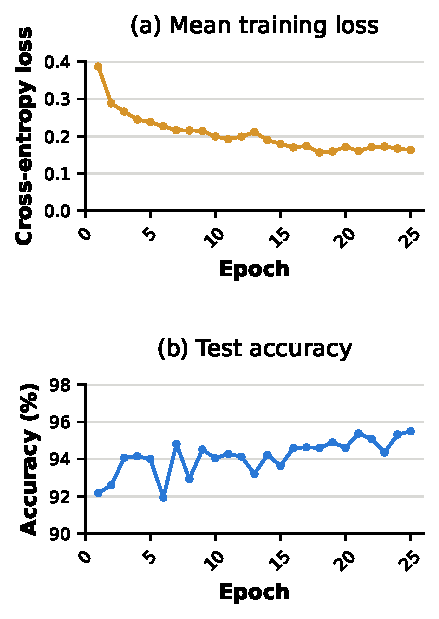
\includegraphics[width=\columnwidth]{fig-training.pdf}
  \caption{Mean training loss (a) and test accuracy (b) per epoch over the
    $25$-epoch run. The accuracy before training (epoch $0$) was $10.08\%$,
    near the $1/10$ chance rate, but is not represented in panel (b), which is
    scaled to the $90\text{--}98\%$ range to show post-training behavior; the
    network reaches its ${\sim}94\text{--}95\%$ plateau within a few epochs and
    finishes at $95.49\%$.}
  \label{fig:training}
\end{figure}

To confirm that the typed network trains as an ordinary classifier, we train it
on the full MNIST training set ($60\,000$ images) for $25$ epochs at a learning
rate of $0.05$ and evaluate on the full $10\,000$-image test set after each
epoch. Test accuracy rises from $10.08\%$ at initialization---near the $1/10$
chance rate, confirming a near-uniform softmax output before training---to
$95.49\%$ after $25$ epochs, while the mean per-example cross-entropy falls from
$0.3871$ to $0.1629$ (\Cref{fig:training}). The network is already on its
${\sim}94\text{--}95\%$ plateau by epoch $3$; from there the epoch-to-epoch
accuracy oscillates within a couple of points (for instance a dip to $91.93\%$
at epoch $6$), the expected behavior of online, batch-size-one SGD with a fixed
learning rate, whose single-example steps nudge the parameters around the
minimum rather than settling exactly into it. For a from-scratch network with no
mini-batching and no BLAS, reaching ${\sim}95\%$ is a functional sanity check
that the typed forward and backward passes are correct end to end, not a
competitive claim.

\subsection{Error analysis}
\label{sec:res:errors}

\begin{figure}[t]
  \centering
  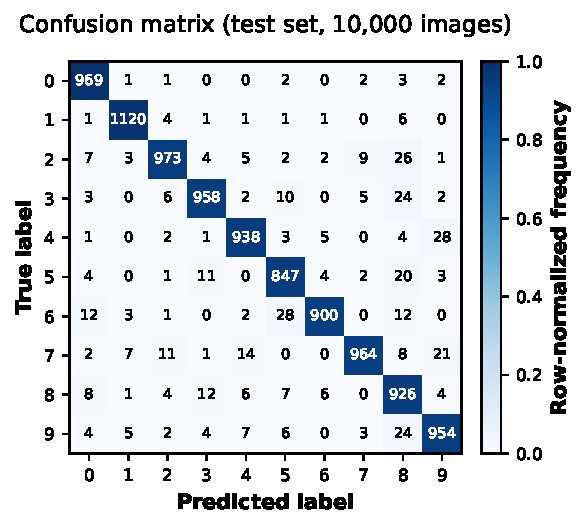
\includegraphics[width=\columnwidth]{fig-confusion.pdf}
  \caption{Confusion matrix on the full $10\,000$-image test set after $25$
    epochs (final accuracy $95.49\%$). Color encodes the row-normalized
    frequency; annotations are raw counts.}
  \label{fig:confusion}
\end{figure}

\Cref{fig:confusion} shows the confusion matrix on the full test set. Most of
the mass lies on the diagonal---which sums to $9\,549$ of $10\,000$, matching
the $95.49\%$ accuracy exactly---but the off-diagonal errors are not spread
uniformly. The most frequently confused pairs are $4\!\to\!9$ ($28$),
$6\!\to\!5$ ($28$), $2\!\to\!8$ ($26$), $3\!\to\!8$ ($24$), $9\!\to\!8$ ($24$),
$7\!\to\!9$ ($21$), and $5\!\to\!8$ ($20$), the visually similar pairs that
MNIST classifiers routinely struggle with. The most revealing pattern is the
column for the digit $8$: it absorbs $127$ false positives---$2$, $3$, $5$, and
$9$ are all commonly misread as $8$---giving it the lowest precision of any
class ($\sim\!87.9\%$). By recall the hardest digits are $7$ ($93.8\%$), $6$
($94.0\%$), and $2$ ($94.3\%$), while $0$ ($98.9\%$) and $1$ ($98.7\%$) are the
easiest, consistent with their distinctive shapes.

\subsection{Scope and limitations}
\label{sec:res:limits}

The evaluation is deliberately modest, matching the project's emphasis on
type-level correctness over throughput. We report a single run at a fixed seed,
so the curves in \Cref{fig:training} carry no error bars and should be read as
indicative rather than as a statistically controlled study. Training uses online
SGD with one gradient step per image, not mini-batches, so the loss curves are
noisier than a batched optimizer would produce, and we make no attempt to tune
the architecture or learning rate for peak accuracy. None of these choices bear
on the correctness claims of \Cref{sec:res:correct}, which are independent of the
seed.

%% =============================================================================
%% 6. Conclusion
%% =============================================================================
\section{Conclusion}
\label{sec:conclusion}

This paper addresses a class of error that ordinarily surfaces only at
runtime---the dimension mismatch between a network's weights, activations, and
gradients---by encoding every tensor's shape in its type. Using type-level
naturals in Haskell, a length-$n$ vector and an $r\times c$ matrix carry their
dimensions as $\mathtt{Nat}$ indices, so an incompatible product, a layer applied
to the wrong-sized input, or two layers composed at a mismatched boundary is
rejected by the compiler rather than crashing at execution. The same discipline
extends to the reverse pass: because the gradient of a tensor has the type of
that tensor, hand-written backpropagation is guarded by the type checker just as
the forward pass is.

The evidence is twofold. The type-level guarantee is demonstrated by the compiler
rejecting a deliberate mismatch before the program runs, and the numerical
content of the implementation is verified by a property-based test suite in which
the hand-derived gradients are checked against finite differences over randomized
inputs (\Cref{sec:res:correct}). As a functional confirmation that the typed
forward and backward passes are correct end to end, the network trains on MNIST
to ${\sim}95\%$ test accuracy with no automatic-differentiation library and no
BLAS (\Cref{fig:training}). The broader takeaway is that a mainstream functional
language, without a specialized dependent type theory, is already expressive
enough to make an entire category of numerical bug unrepresentable, and to do so
without hiding the mathematics inside a framework.

The scope of the work is deliberately narrow. The architecture is a single
two-layer classifier trained with online SGD on MNIST, and the
emphasis on type-level correctness comes at the cost of throughput: boxed vectors
with no BLAS make a full $25$-epoch run over the $1.5$~million per-example steps
take on the order of hours rather than the seconds a batched, BLAS-backed
implementation would need. These are boundaries of the demonstration, not of the
technique. The natural next step is
to generalize the typed core from a fixed two-layer network to an arbitrary stack
of layers---representing a network as a type-level list of dimensions and folding
the forward and backward passes over it---so that networks of any depth inherit
the same compile-time shape guarantee. Extending the shaped primitives to
mini-batches and to an unboxed representation would then close the gap between
the correctness demonstrated here and practical performance.

%% =============================================================================
\bibliographystyle{ACM-Reference-Format}
\bibliography{references}

\end{document}